
% Many thanks to Andrew West for writing most of this file
% Main LaTeX file for CIS400/401 Project Proposal Specification
%
% Once built and in PDF form this document outlines the format of a
% project proposal. However, in raw (.tex) form, we also try to
% comment on some basic LaTeX technique. This is not intended to be a
% LaTeX tutorial, instead just (1) a use-case thereof, and (2) a
% template for your own writing.

% Ordinarily we'd begin by specifying some broad document properties
% like font-size, page-size, margins, etc. -- We have done this (and
% much more) for you by creating a 'style file', which the
% 'documentclass' command references.
\documentclass{sig-alternate}

% These 'usepackage' commands are a way of importing additional LaTeX
% styles and formattings that aren't part of the 'standard library'
\usepackage{mdwlist}
\usepackage{url}

\begin{document}
\nocite{*}
% We setup the parameters to our title header before 'making' it. Note
% that your proposals should have actual titles, not the generic one
% we have here.
\title{Electronic Knee Wrap for Injury Prediction}
\subtitle{Dept. of CIS - Senior Design 2013-2014\thanks{Advisor: LeAnn Dourte (dourte@seas.upenn.edu), Insup Lee (lee@cis.upenn.edu)}}
\numberofauthors{4}
\author{
\alignauthor Alex Yau \\ \email{ayau@sas.upenn.edu} \\ Univ. of Pennsylvania \\ Philadelphia, PA
\alignauthor Jacy Clare \\ \email{jclare@sas.upenn.edu} \\ Univ. of Pennsylvania \\ Philadelphia, PA
\and
\alignauthor Jeffrey Shih \\ \email{jeshih@sas.upenn.edu} \\ Univ. of Pennsylvania \\ Philadelphia, PA
\alignauthor Kunal Mahajan \\ \email{mkunal@seas.upenn.edu} \\ Univ. of Pennsylvania \\ Philadelphia, PA}
\date{\today}
\maketitle

% Next we write out our abstract -- generally a two paragraph maximum,
% executive summary of the motivation and contributions of the work.
\begin{abstract}

  \textit{Anterior Cruciate Ligament (ACL) injuries are among the most common injuries in sports. While significant research has been conducted for identifying the factors responsible, there is a need to quantitatively determine an athlete's risk of suffering the injury in real time. To this end, we explore the opportunity to mount a high performance, small area circuit on a knee wrap. We integrate a set of factors such as knee acceleration, knee orientation and valgus forces for computing the risk percentage of an athlete in real time. In addition, this knee wrap will also be multi-purpose, allowing both doctors to predict injuries and athletes prevent injuries on the field.}

  \textit{The design incorporates microcontrollers, inertial measurement units and wireless module mounted on the knee wrap. In order for the therapists and physicians to interact with the data, we have implemented a server and are using a website to display the data. We are able to show that the sensors measure accurate data at (TODO Hz) frequency, successfully transmit to the server and display the data.}

\end{abstract}

\begin{keywords}
	Anterior Cruciate Ligament (ACL),  Knee Flexion angle, Deceleration, Knee Injury Risk Index (KIRI)
\end{keywords}

% Then we proceed into the body of the report itself. The effect of
% the 'section' command is obvious, but also notice 'label'. Its good
% practice to label every (sub)-section, graph, equation etc. -- this
% gives us a way to dynamically reference it later in the text via the
% 'ref' command.
\section{Introduction}
\label{sec:intro}
ACL ruptures are one of the most common injuries in sport and very expensive to treat.There are approximately 175, 000 primary ACL reconstruction surgeries performed annually in the USA with an estimated cost of over \$2 billion US \cite{yu2007mechanisms}. This is followed by a lengthy rehabilitation period. Even then, over a quarter of patients reinjure their ACL \cite{stevenson1998gender}. These injuries also cause early-onset of osteoarthritis for numerous people between the ages of 30 and 50, and related injuries such as ACL tear in the other leg. (TODO cite Lohmander et al)

An ACL injury can have an immense impact on an athelete's career and quality of life. Because of this, preventing ACL injuries is exceptionally valuable and important. We propose the use of an electronic knee wrap (eKwip), to predict and prevent ACL injuries in both healthy athletes and injured patients. By monitoring the angles, orientation and movements of the knee of the wearer, eKwip is able to predict when an injury is imminent. We propose to create a prevention mechanism to cushion knee and prevent the knee from bending at angles that may cause an ACL rupture. This mechanism will be triggered in case of imminent danger. To encourage adoption of such a knee wrap, eKwip is designed to be unobtrusive and flexible, unlike the current mechanical braces on the market.

eKwip allows the wearer to monitor his or her knee performance and risk of injury throughout the day to decrease the chance of future injury. It also allows physical therapist to easily observe and assess the performance of injured patients remotely. With eKwip, the aim is to reduce the rate of ACL injuries in both healthy athletes and injured patients.

eKwip utilizes various factors that have been demonstrated to cause the injury such as accelerations and angles. It integrates these factors with machine learning algorithm to accurately calculate the risk by adapting to the athlete's physical characteristics such as flexiblity and normal range of knee movement. Currently, the microcontroller (Mbed) receive knee acceleration and orientation angles from the sensors. Using a wireless module, this data is quickly transmitted to the server, which calibrates the angles and acceleration, and displays them on the website in a user friendly format.

Sec.2 reviews knee anatomy, including the major causes of ACL injuries and the performance requirement of eKwip. Then, we review the prior work in ACL detection and the common rehabilation procedures used in the industry for measuring the strength of the ACL in Sec.3. Sec.4 illustrates the basic idea of eKwip with the model diagram. Sec.5 describes the technical implementation of eKwip in detail. As real-time analysis is a necessary component, Sec.6 describes the performance of the system with respect to requirements and how we improved the system over time. Sec.7 details our remaining work that involves implementation of KIRI algorithm, machine learning implementation, and testing and validating the system. Throughout the paper, we focus on latency and unobtrusiveness of the wrap.

% The header of this document might have been a little intimidatating
% to beginners. Notice once you are in the body of the document,
% however, LaTeX commands are minimal and 'normal text' is frequent.
\section{Background}
\label{sec:background}
\subsection{Knee Joint and ACL} 
As the paper includes interdisciplinary content, it is necessary to first provide information in this section about the mechanical properties of the knee used throughout the paper. The knee joint is the largest joint in the human body that connects the femur and tibia. ACL is one of the four major ligaments in the knee. It originates from deep within the lower extremity of the femur and attaches in front of the spine of tibia. The Figure~\ref{fig:knee_anatomy} below is representative of the knee anatomy and the location of ACL. 

\begin{figure}[h]
  \begin{center}
    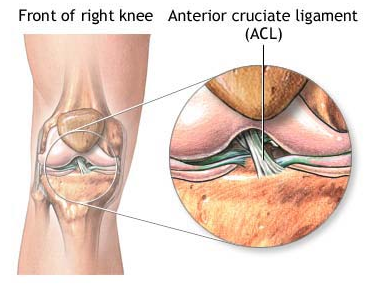
\includegraphics[width=3in]{images/acl_anatomy.bmp}
  \end{center}
  \caption{Knee anatomy and location of ACL}
  \label{fig:knee_anatomy}
\end{figure}

\subsection{Knee Flexion Angles}
ACL is responsible for resisting anterior translation and medial rotation of the tibia, in relation to the femur. This resistance is crucial for controlling the forward movement and twisting of the knee. Major cause of ACL injury is small knee flexion angle along with medial rotation. The knee flexion angle is the angle between the femur and the tibia. The medial rotation is the internal rotation of the knee towards the midline axis of the human body. As a result, these angles are an important indicator for the injury.

\subsection{Asymmetric distributed forces}
Another common reason for the ACL injury is due to asymmetric distributed forces acting on the joint. As these forces are not equally distributed, the resultant force direction does not pass through the vertical axis at the center of the leg. This resultant force causes anterior translation and medial rotation. Once the forces exceed the resistance offered by the ACL,  the ACL ruptures due to excessive strain (TODO cite GRIFFIN et al). Now, these forces are caused due to sudden movements such as changing directions or landing from a jump, which are most common in sports (TODO cite GRIFFIN et al). These decelerations generally happen as fast as 50ms (TODO cite some paper), and therefore, ekwip needs to be able to measure the deceleration as fast as 10s of milliseconds. The decelerations can then be related to the forces to provide a more complete analysis for risk calculations.

\section{Related Work}
\label{sec:related_work}
Related work for this project is divided among three fields: algorithms for ACL injury detection (Section 2.1), knee brace effectiveness/performance hindrance (Section 2.2), and Smart Materials (Section 2.3). ACL injury detection covers previous research in minimizing the testing required to detect whether an athlete is at risk of suffering an ACL injury. Knee brace effectiveness/performance hindrance deals mainly with studies of the extent to which a Functional Knee Brace and a Prophylactic Knee Brace play in the ability for an athlete to perform on the field. Finally, Smart Materials concern the reach for this project and the possibility of actually preventing the ACL injuries from occurring on the field.

\subsection{ACL Injury Detection} Prior research in ACL Injury Detection have shown that techniques exist that accurately capture and analyze various measures relating to the knee to determine the probability of ACL injuries \cite{smedicine}. Using such metrics as knee valgus motion, knee flexion rotation of motion, and body mass, researchers were able to come up with a way to determine knee abduction moments (KAM), which are used to identify whether or not an athlete is at high risk for an ACL injury, with a sensitivity of 77\% and specificity of 71\% \cite{smedicine}\cite{Bahr01062005}. 

\subsection{Knee Brace Effectiveness/ Performance Hindrance} Prior research in using Functional or Prophylactic knee braces out in the field useful but results on the potential hindrance of using these kinds of braces were inconclusive \cite{Myer01042011}. Knee braces, especially Functional Knee Braces (FKB), which are more mechanical in nature and thus more obtrusive, are shown to provide “20-30\% greater knee ligament protection”. This suggests that FKBs have an impact in reducing the severity of knee injuries. More testing needs to be done to see whether or not FKBs will actually hinder the performance of an athlete. Another important factor of the effectiveness of knee braces is in rehabilitation, where a combination of exercises and brace use can speed up recovery \cite{hewett2010acl} .

\subsection{Smart Materials} Prior research in the use of Electro-rheological fluids (ERF) show that these material reacts quickly when presented with an electric field, have a high yield stress, and are very lightweight and easily molded \cite{smaterials}. ERF can quickly change viscosities, which make it an excellent material to use in the project. Due to the very nature of ERF’s fast response and simple interface, using it in a light, functional knee brace would allow lead to an easy implementation of the preventative nature of the project.

\section{System Model}
\label{sec:system_model}
Talk briefly in high level about the model.
Include the flow chart that we made.
talk about how stuff interacts
avoid lot of technical implementation in this section as the next section talks about the implementation in detail

\section{System Implementation}
\label{sec:system_implementation}
eKwip consists of several components that all work together to collect data about the position and motion of the knee and leg, send the data over a wireless network link to a server, and analyze the data in order to display an image of the knee and collect comprehensive data regarding the motion of the knee.

The process begins in the IMU sensors, which use accelerometers and gyroscopes to measure the absolute orientation, acceleration, and rate of change of acceleration. This data is passed to the microcontroller, which packetizes the data and sends it to the wireless module. The Wifly then transmits the data packets over the wireless network to the server.

The server receives the data packets and parses the data. It then computes the position and movement of the knee in order to display the image of the leg in the graphical user interface and record the position and motion data in a file on the server, which can be used for graphing and further analysis.

\subsection {Spandex Wrap}
eKwip is a spandex wrap that fits around the leg, above and below the knee. A wrap of this type was chosen because it's relatively small, unobtrusive, and stays close to the skin, which is important for correctly measuring the movement of the knee itself, instead of the movement of the wrap. The wrap was designed to be unobtrusive in order to encourage athletes to wear it more often. Unlike current mechanical braces on the market, eKwip does not hinder the movement of the knee, which makes eKwip much more attractive to athletes.

\subsection {mBed Microcontroller}
The microcontroller is responsible for reading data from the sensors and sending the data over the network link. A microcontroller was chosen based on storage capacity, clock speed, ease of use, and the ability to multitask. These are important because a fast processor will allow the reading of data at a high frequency, a decent amount of storage will facilitate the storage of the code libraries in use and to give some initial storage for the data, and the ability to multitask will enable the reading of data and send it over a network link simultaneously. Given all these considerations, the mBed LPC1768~\cite{mbed} was selected as an ideal microcontroller for this project.

The mBed is ideal for this project because of its small size and impressive performance. Perhaps most importantly, the mBed has the ability to interface with many different modules at the same time, as it includes three UART serial ports, two SPI ports, two I2C ports, a USB port, a CAN port, and an ethernet port, among other GPIO pins. The mBed contains a powerful 96 MHz ARM Cortex-M3 processor. These features come together to allow several sensors and communication devices to be connected to the mBed at one time.

\subsection {UM6-LT Sensors}
In addition to the microcontroller, eKwip also requires sensors to collect information from the wearer's knee. A set of two inertial measurement units, or IMUs, were selected for this purpose. Two IMUs are required, one on the upper leg and one on the lower leg, so the relative angles of the knee can be measured in order to give an accurate model of the leg. A small IMU that is able to send data very quickly and communicates via UART serial is utilized by eKwip. This allows easy mounting of the IMUs, fast data reading, and easy interface with the mBed. In accordance with all of these considerations, the Pololu UM6-LT~\cite{um6} was chosen as the best IMU for this application. The UM6-LT is approximately the size of a quarter, and can measure absolute angles, rate of change of the angles, and acceleration.

An mBed library for the sensors was initially used in order to set up the IMUs and get initial data readings. However, once performance became a concern, it was clear that the library would not give the speed required for the prediction of ACL injuries. The UM6-LT offers two operating modes, broadcast and query. The library used query mode, which involves sending a query to the IMU and waiting for a response. This was the limitation in the speed, so a new library was implemented, which utilizes the UM6-LT's broadcast mode. This allows much faster reading, on the order of 3$\mu$s per data point, as opposed to the previous read time of 30$\mu$s.

\subsection {Wifly Wireless Module}
In order to allow coaches to monitor the performance of athletes on the field and doctors to monitor the recovery of injured patients, a wireless interface that allows eKwip measurements to be displayed in real time was implemented. In order to achieve wireless communication, a Wifly module~\cite{wifly} was integrated into the system. The Wifly is a small Wifi board that communicates via UART serial. Having a wireless connection is useful because data can be streamed in real time to the server that is running in order to provide an intuitive visualization to users and/or their doctors. The only constraint with this is that the user must be in range of a wireless network.

The Wifly is configured to send a packet each time a data point is received. This, along with an increased baud rate on the serial line between the mBed and the Wifly module, allowed for a wifi sampling rate of up to 100 Hz.

\subsection {Node.js Server}
The server is implemented with Node.js~\cite{node} and communicates with the eKwip wrap via websockets~\cite{websockets}. Websockets were chosen in order to provide a stream of information from the wrap to the server. The server collects the data streamed from the wrap and in turns communicates to the front-end interface. Some simple logic is implemented on the server to normalize and calibrate the data sent from the wrap, as well as filter out possible measurement errors. The front-end currently displays a 3D model of the knee given the data from eKwip with WebGL~\cite{webgl}. However, in the future, the front-end will also allow multiple users to log in to view indivisualized reports and statistics, and share this information with their physician. This can allow patients and doctors to monitor the performance of the knee as well as observe the recovery of a patient over time.


\section{System Performance}
\label{sec:system_performance}
In order to correctly predict ACL injuries in real time, data must be collected at a certain frequency so that subtle movements and accelerations are captured in the data. When the sensors were first integrated with the mBed, the rate at which data could be read was not fast enough. Therefore, problems in the library being used were identified and rectified.

Another problem with the performance was the network latency. At first, the data was being transmitted over the network in discrete packets, each several seconds apart. It was determined that the wifi module was buffering the data until a large enough packet was received before transmitting the packet. This was mitigated by configuring the wifi module to send data after each receipt of a data packet. However, the transmission rate still was not fast enough, which required the shortening of the data string used to communicate each data point.

The improvements in data sampling and network transmission rates can be seen in Figure~\ref{fig:graph}.

\begin{figure}[h]
  \begin{center}
    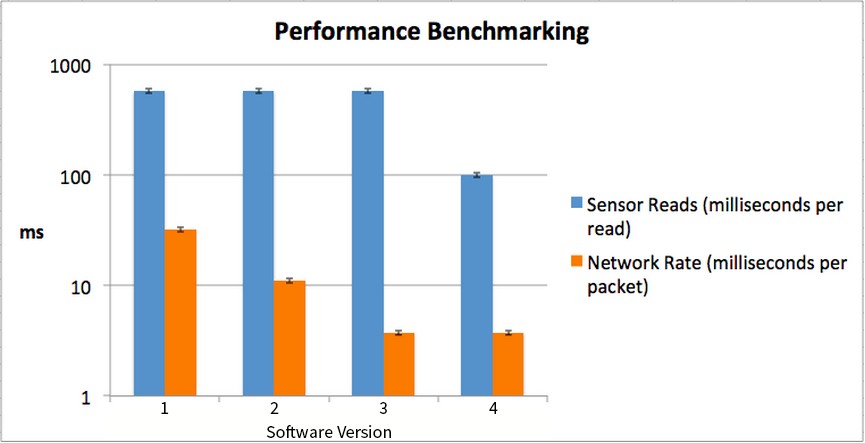
\includegraphics[width=3in]{images/graph.png}
  \end{center}
  \caption{Network and sensor performance of various eKwip prototypes}
  \label{fig:graph}
\end{figure}


\section{Remaining Work}
\label{sec:remaining_work}
At its current point, eKwip is in the prototype stage. While the current implementation is able to collect data on the wearer's knee movements as well as transmit that data to the server, there is no conclusive metric being calculated for the prototype. As such, the first step moving forward is to come up with an algorithm to calculate the Knee Injury Risk Index (KIRI). In order to do this, certain factors, such as the calculated Q-angle or knee adduction moment during movement, after being calculated, will be given certain weights and a final KIRI value will be returned for the wearer. The Q-angle is formed from a line drawn from the Anteriro Superior Iliac Spine (the front of the pelvic bone at the hip level) to the center of the kneecap, and from the center of the kneecap to the Tibial Tubercle (a bump about 5 centimeter below the kneecap on the front of the Tibia \FIXME{Add a citation for this}. The knee adduction moment determines how force is distributed at the knees \FIXME{Add citation}. A higher Q-angle means that the wearer has an increased risk of ACL injuries, while the knee adduction moment of a person in movement will affect how certain loads are applies to their knees and ACL. 

Another important issue that needs to be addressed is the variability of gaits, resting positions, and Q-angles from person-to-person. Designing a wrap that fits everyone will not generate accurate results as we move between athletes. Our solution to this issue is to produce a basic machine learning algorithm that will cause eKwip to adapt to wearer. The algorithm will likely collect data on the wearer initially. Then, using this information, eKwip will adjust its collection formulas to fit with how the wearer normally rests or moves. This aspect of the project will likely be the most difficult; therefore, we will be spending a major portion of the remaing time on creating and validation the implementation.

Testing and validation of all data collection and the system itself will be carried out along with the implementation of the previously mentioned features. Validation is critical for the system and will make-or-break whether or eKwip is actually useful as an aid for physical therapists or coaches. Fortunately, access to equipment at the Penn Sports Medicine Center will allow us to test eKwip against what is currently being used. Because of the nature and focus of our project, certain data will be very risky or even dangerous to collect on an actual person. Fortunately, knee models at the Penn Sports Medicine Center will allow us to collect this information as well as give us methods to gather data on the knee in various positions or stances. Moving forward, testing and validation will be continually done, with majors tests performed when major milestones are completed on the project.

Based on how fast these features can be implemented and how much time remains, we may pursue the reach goal: to implement a prevention measure for eKwip that will be an extension of the prediction. However, this largely depends on how fast we can perform reads and calculations on the system itself as well as how quickly we can ensure the accuracy of the values. Prevention also requires major research into potential materials to use, as eKwip would need a method to brace the sudden movement of the wearer to lessen or prevent the injury. In addition, a Prevention implementation will modify the rate and method of data collection and calculation. It is likely we may not reach this stage of the project, but, as stated, this is all highly dependent on the time constraints. 

% We next move onto the bibliography.
\bibliographystyle{plain} % Please do not change the bib-style
\bibliography{sections/references}  % Just the *.BIB filename

\end{document}

